\documentclass[border=12pt]{standalone}
\usepackage[utf8]{vietnam}
\usepackage{times}
\usepackage{tikz}
\usetikzlibrary{arrows.meta,calc}

\begin{document}
\begin{tikzpicture}
  % Base image
  \node[anchor=south west,inner sep=0] (image) at (0,0) {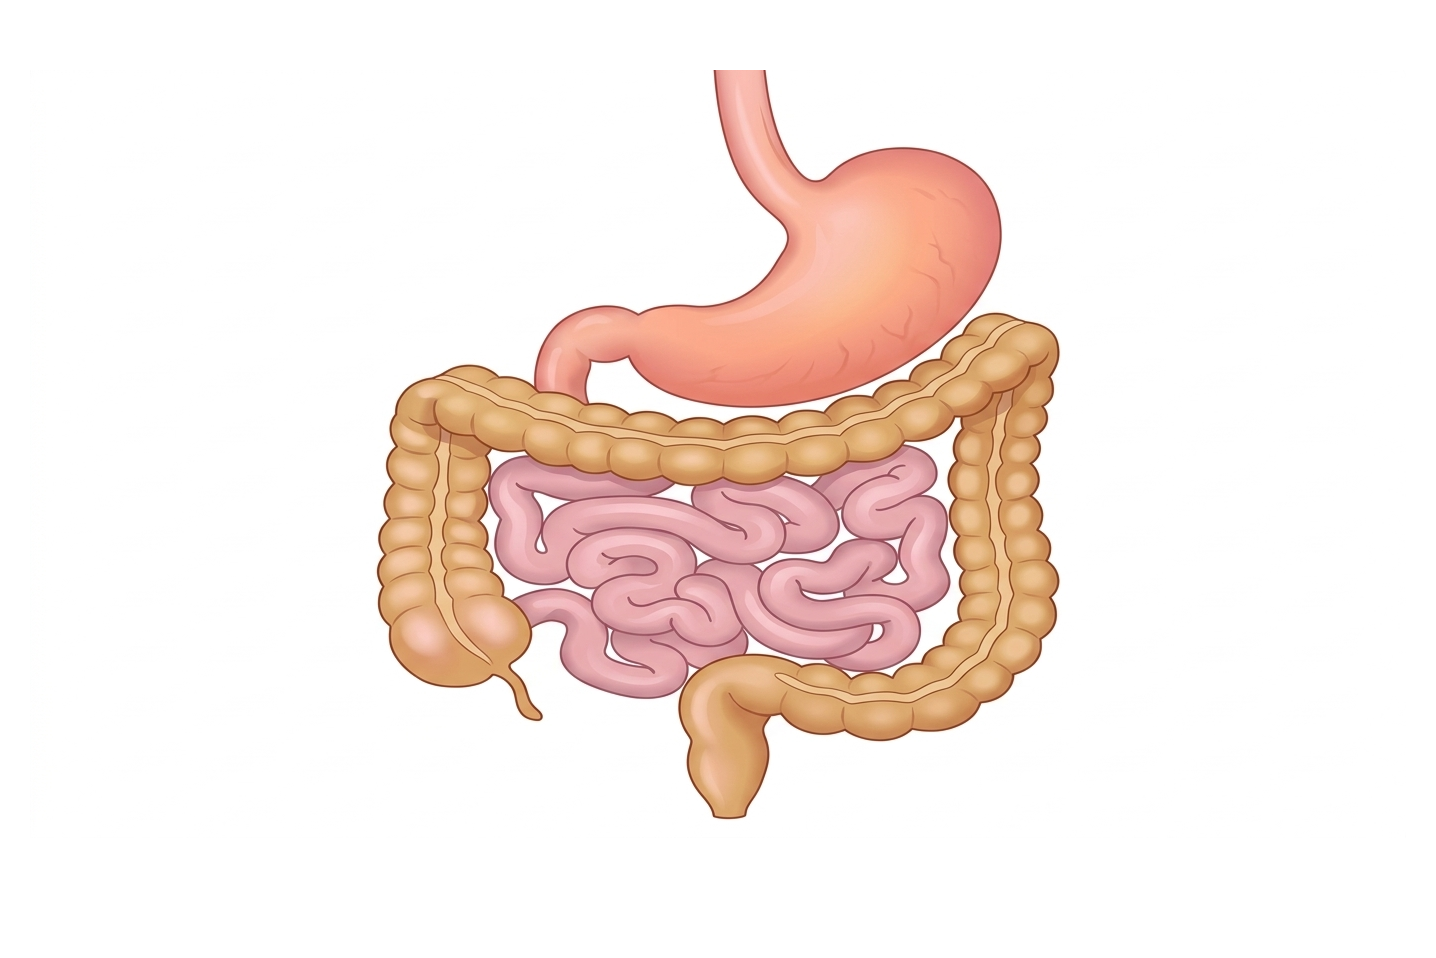
\includegraphics[width=15.5cm]{padded_exact.png}};
  \begin{scope}[x={(image.south east)},y={(image.north west)}]

    % Styles
    \tikzset{
      lbl_title/.style={font=\fontsize{12pt}{15pt}\selectfont\bfseries, inner sep=1pt},
      lbl_ph/.style={font=\fontsize{11.5pt}{14.5pt}\selectfont\bfseries, text=blue!85!black, inner sep=1pt},
      arrow_style/.style={-{Stealth[scale=1.15, length=6pt, width=4.5pt]}, line width=1.1pt, draw=black!90}
    }

    % 1. Khoang miệng (Top-Left)
    \node[anchor=east, align=center] (lbl_mieng) at (0.39, 0.93) {
      {\fontsize{12pt}{15pt}\selectfont\bfseries Khoang miệng}\\[2pt]
      {\fontsize{11.5pt}{14.5pt}\selectfont\bfseries\color{blue!85!black} pH 6,5 -- 7,5}
    };
    \draw[arrow_style] (lbl_mieng.east) -- (0.505, 0.925);

    % 2. Khoang dạ dày (Upper-Left above stomach)
    \node[anchor=east, align=center] (lbl_daday) at (0.43, 0.78) {
      {\fontsize{12pt}{15pt}\selectfont\bfseries Khoang dạ dày}\\[2pt]
      {\fontsize{11.5pt}{14.5pt}\selectfont\bfseries\color{blue!85!black} pH 1,5 -- 3,5}
    };
    \draw[arrow_style] (lbl_daday.east) -- (0.54, 0.72);

    % 3. Tá tràng (Left)
    \node[anchor=east, align=center] (lbl_tatrang) at (0.24, 0.63) {
      {\fontsize{12pt}{15pt}\selectfont\bfseries Tá tràng}\\[2pt]
      {\fontsize{11.5pt}{14.5pt}\selectfont\bfseries\color{blue!85!black} pH 5,6 -- 8,0}
    };
    \draw[arrow_style] (lbl_tatrang.east) -- (0.375, 0.585);

    % 4. Ruột non (Right)
    \node[anchor=west, align=center] (lbl_ruotnon) at (0.76, 0.44) {
      {\fontsize{12pt}{15pt}\selectfont\bfseries Ruột non}\\[2pt]
      {\fontsize{11.5pt}{14.5pt}\selectfont\bfseries\color{blue!85!black} pH 7,2 -- 7,5}
    };
    \draw[arrow_style] (lbl_ruotnon.west) -- (0.58, 0.395);

    % 5. Ruột già (Right - lower)
    \node[anchor=west, align=center] (lbl_ruotgia) at (0.76, 0.28) {
      {\fontsize{12pt}{15pt}\selectfont\bfseries Ruột già}\\[2pt]
      {\fontsize{11.5pt}{14.5pt}\selectfont\bfseries\color{blue!85!black} pH 7,9 -- 8,5}
    };
    \draw[arrow_style] (lbl_ruotgia.west) -- (0.645, 0.285);

    % 6. Caption at bottom
    \node[anchor=center] at (0.50, 0.05) {
      {\fontsize{13pt}{16pt}\selectfont\bfseries Hình. pH trong hệ tiêu hoá của con người}
    };

  \end{scope}
\end{tikzpicture}
\end{document}
